\section{Experimental setup and Procedure}
\subsection{The two methods}
For the experiment we use two different methods to analyze the
resonance frequency.
\begin{figure}[htpb]
    \centering
    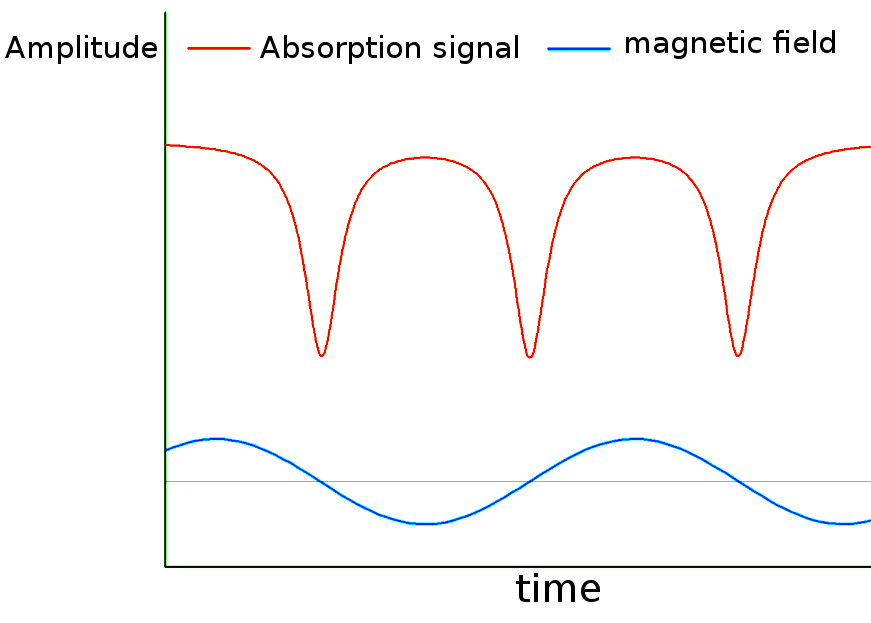
\includegraphics[width=0.7\linewidth]{figures/method1}
    \caption{As you see the minima of the adsorption signal lie within
        the roots of the magnetic field amplitude (Figure
            taken from~\cite{versuchsanleitung} and changed).}
    \label{fig:method1}
\end{figure}
\paragraph{Method 1} First we use a method which consists on applying a 
sinus curved magnetic field with known frequency to the sample. 
The main point is that have an inner RLC-circuit creates an electromagnetic
wave field inside of the sample. When the frequency of the field attaches
the absorption line of the nuclear spin, this influence will be measurable
at the circuit by means of its damping factor. By construction the 
amplitude will be lower and we can conclude the frequency. This will
be the case periodically since we forced the magnetic field to a 
sinusoidal signal. The resulting curve is visualized 
in figure~\ref{fig:method1}. \\\\
\paragraph{Method 2} 
\begin{figure}[htpb]
    \centering
    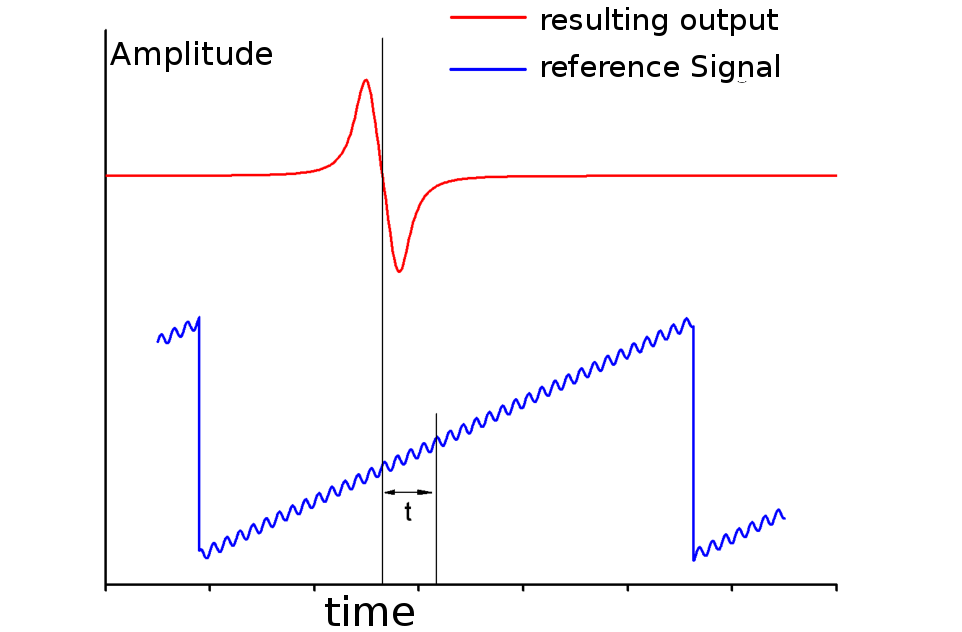
\includegraphics[width=0.8\linewidth]{figures/lockin2}
    \caption{Reference and resulting signal with the lockin method
        (changed from \cite{versuchsanleitung}).}
    \label{fig:lockin2}
\end{figure}
In this method we use sawtooth curve, modulated
with a sinus for the magnetic field:
\begin{equation}
   U(t) = U_{sz} \left[ t - \lfloor t \rfloor \,  \right] + U_0 \sin(\omega t)
\end{equation}
where the $\lfloor t \rfloor$ denotes to the gauss bracket (rounding down). 
\begin{figure}[htpb]
    \centering
    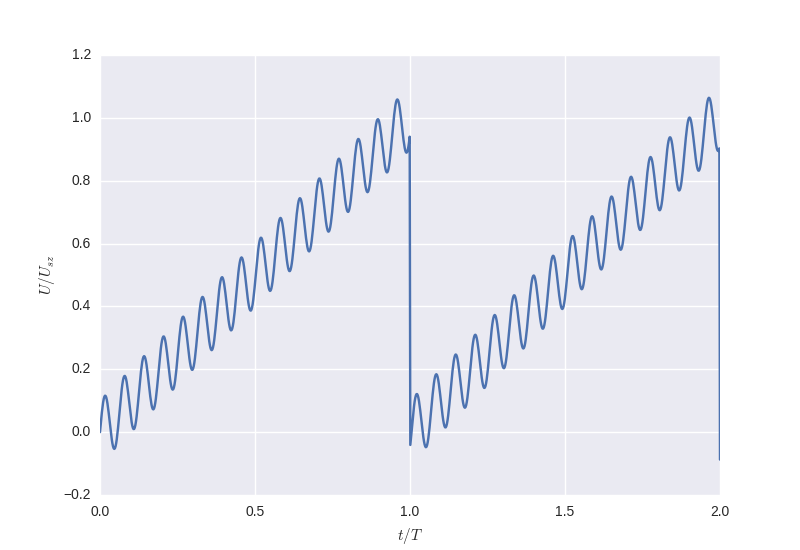
\includegraphics[width=0.8\linewidth]{figures/sawtooth}
    \caption{Reference signal for our lockin amplifier}
    \label{fig:sawtooth}
\end{figure}
We use the sawtooth curve to find the frequency, which will be 
realized as the derivate of a peak.
\subsubsection{Procedure}
\label{ssubsec:procedure}
In order to derive the magnetic moments and gyromagnetic ratios, 
we use the relationship to applied magnetic fields given by the Zeeman effect 
as established in the theory section \ref{sec:theory)}. 
The point of resonance leads to the appearance of absorption lines 
in the strength of the highly oscillating field. These absorption lines 
will then be measured. 
The steps undertaken in this experiment are the following:
\begin{enumerate}
\item
measuring the homogenity of the magnetic field in order to define a stable working point;
\item
measuring the resonance frequency for a given external magnetic field by searching for 
equidistant absorption peaks;
\item
measuring the resonance frequency with a lock-in amplifier and sine modulated saw tooth signal.
\end{enumerate}
From the obtained data, we then calculate the following quantities:
\begin{enumerate}
\item
nuclear magnetic moment of $^19$F;
\item
gyromagnetic moment of proton in $^1$H, glycole and fluor.
\end{enumerate}

\begin{figure}[htpb]
    \centering
    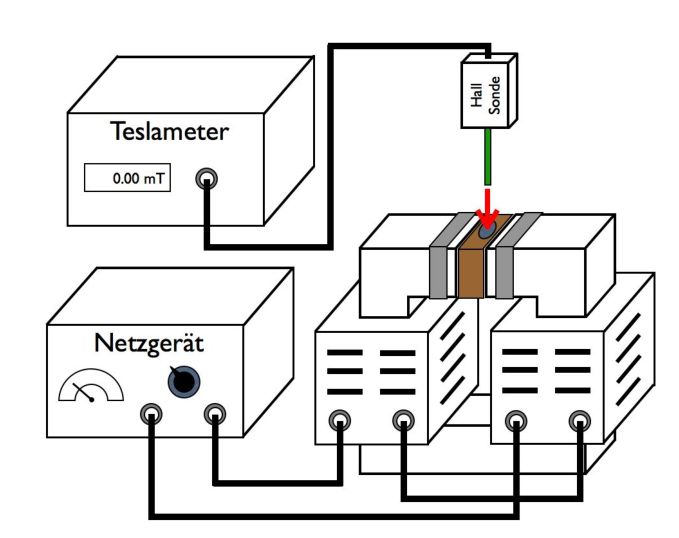
\includegraphics[width=0.8\linewidth]{figures/setup1}
    \caption{\textbf{Step 1:} Measuring the magnetic field with the help of 
       an hall effect sensor. As you can notice from the figure we 
      apply various Potentials, which cause an current in the coil which
      further results in an magnetic field sensing by the hall effect sensor
      ~\cite{versuchsanleitung}.}
    \label{fig:figures/setup1}
\end{figure}
\begin{figure}[htpb]
    \centering
    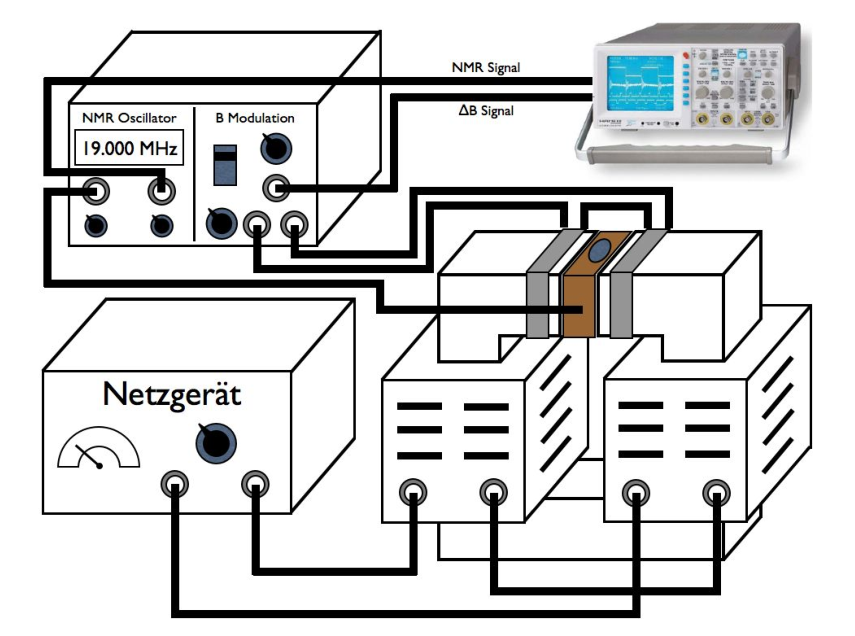
\includegraphics[width=0.8\linewidth]{figures/setup2}
    \caption{\textbf{Step 2:} Measuring the resonance frequency with the first
        method. You notice that we do not use the lockin amplifier yet,
        this will be the case in the following steps, instead we vary the
        frequency with constant current and voltage in oder to observe
        the periodic peaks as already described~\cite{versuchsanleitung}. }
    \label{fig:figures/setup1}
\end{figure}
\begin{figure}[htpb]
    \centering
    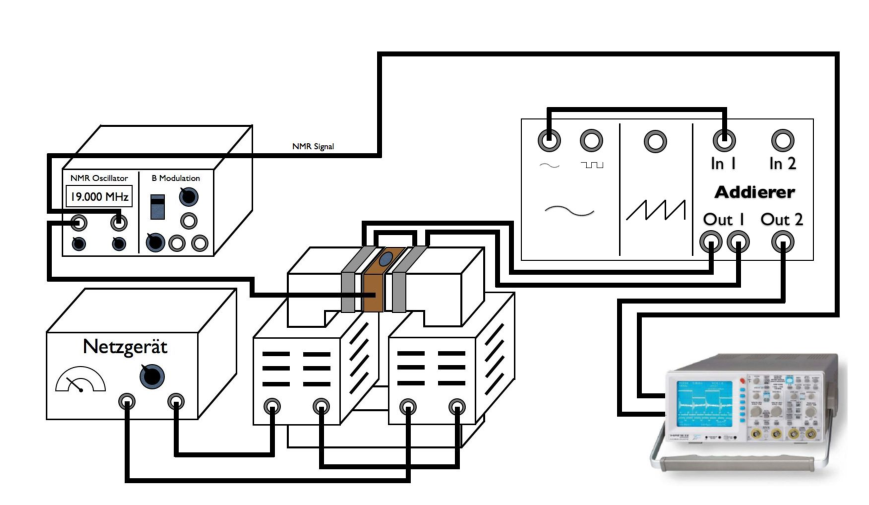
\includegraphics[width=0.8\linewidth]{figures/setup3}
    \caption{\textbf{Step 3:}
        We used this experimental setup to calibrate the following
        measurements~\cite{versuchsanleitung} such that we are already
        near the resonance frequency in order to resolve it with an high
        precision.}
    \label{fig:figures/setup1}
\end{figure}
\begin{figure}[htpb]
    \centering
    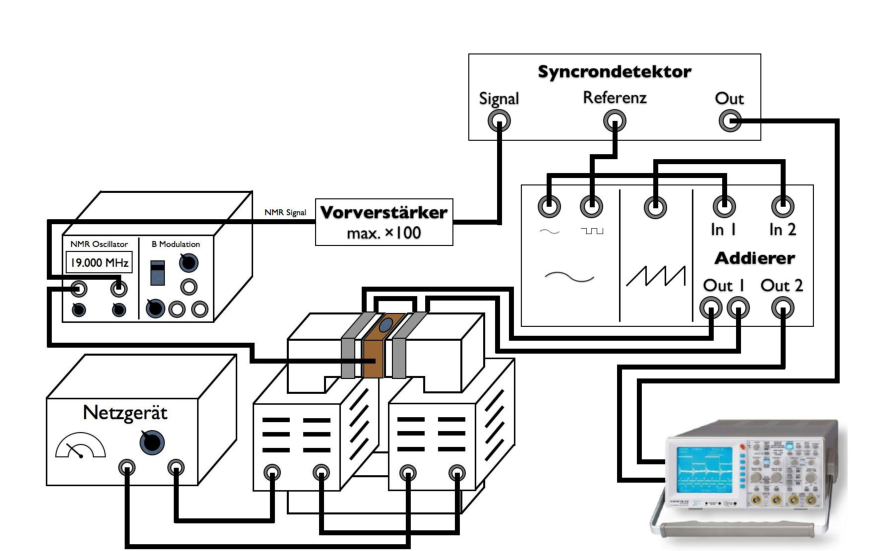
\includegraphics[width=0.8\linewidth]{figures/setup4}
    \caption{\textbf{Step 4:}
        Finally we can use this experimental setup to measure
        the resonance frequency with the lockin method~\cite{versuchsanleitung}.}

    \label{fig:figures/setup1}
\end{figure}
\clearpage




